
\section{Prueba 2}


\subsection{Red de inferencia}
\begin{center}
	\tikzstyle{regla}= [rectangle,draw,black,fill=blue!15]
	\tikzstyle{hecho}= [rectangle,draw,black,fill=black!15]
	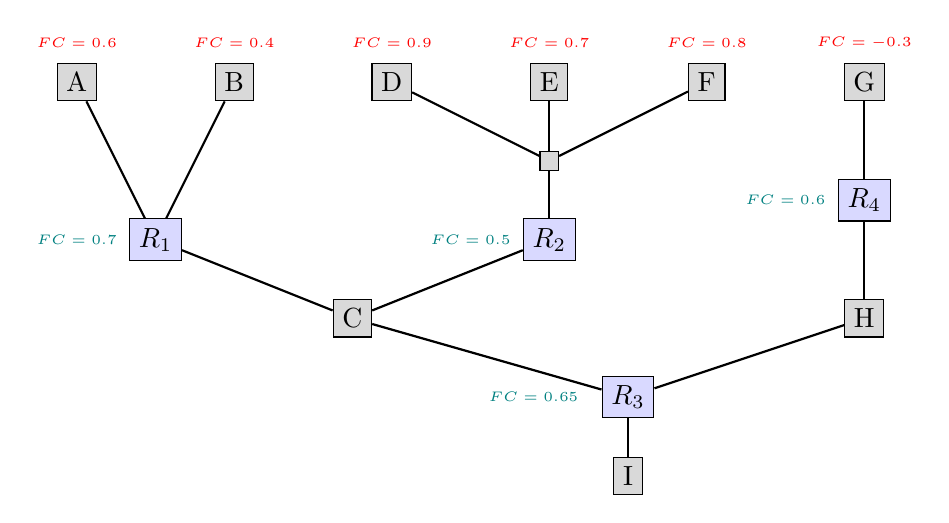
\begin{tikzpicture}
		\node (a) at (0,5) [hecho] {A};
		\node at (0,5.5) {\color{red}{\tiny{$FC=0.6$}}};

		\node (b) at (2,5) [hecho] {B};
		\node at (2,5.5) {\color{red}{\tiny{$FC=0.4$}}};

		\node (c) at (3.5,2) [hecho] {C};

		\node (d) at (4,5)[hecho] {D};
		\node at (4,5.5) {\color{red}{\tiny{$FC=0.9$}}};

		\node (e) at (6,5)[hecho] {E};
		\node at (6,5.5) {\color{red}{\tiny{$FC=0.7$}}};

		\node (f) at (8,5)[hecho] {F};
		\node at (8,5.5) {\color{red}{\tiny{$FC=0.8$}}};

		\node (g) at (10,5)[hecho] {G};
		\node at (10,5.5) {\color{red}{\tiny{$FC= -0.3$}}};

		\node (h) at (10,2)[hecho] {H};

		\node (i) at (7,0)[hecho] {I};

		\node (d/e/f) at (6,4)[hecho] {};

		\node (r1) at (1,3) [regla] {$R_{1}$};
		\node at (0,3) {\color{teal}{\tiny{$FC=0.7$}}};
		\node (r2) at (6,3) [regla] {$R_{2}$};
		\node at (5,3) {\color{teal}{\tiny{$FC=0.5$}}};
		\node (r3) at (7,1) [regla] {$R_{3}$};
		\node at (5.8,1) {\color{teal}{\tiny{$FC=0.65$}}};
		\node (r4) at (10,3.5) [regla] {$R_{4}$};
		\node at (9,3.5) {\color{teal}{\tiny{$FC=0.6$}}};

		\path[black,thick] (a) edge[] node {} (r1);
		\path[black,thick] (b) edge[] node {} (r1);
		\path[black,thick] (r1) edge[] node {} (c);
	
		\path[black,thick] (d) edge[] node {} (d/e/f);
		\path[black,thick] (e) edge[] node {} (d/e/f);
		\path[black,thick] (f) edge[] node {} (d/e/f);
		\path[black,thick] (d/e/f) edge[] node {} (r2);
		\path[black,thick] (r2) edge[] node {} (c);

		\path[black,thick] (g) edge[] node {} (r4);
		\path[black,thick] (r4) edge[] node {} (h);

		\path[black,thick] (c) edge[] node {} (r3);
		\path[black,thick] (h) edge[] node {} (r3);
		\path[black,thick] (r3) edge[] node {} (i);


		\end{tikzpicture}
\end{center}


\subsection{Objetivo obtenido por SBR-FC}

\subsection{Cuestión}
\begin{ejer}
	\textbf{Prueba 2.} En un momento determinado se tiene la siguiente información sobre los hechos:\\
	Se está cumpliendo \texttt{A} con grado 0.6, \texttt{B} con grado 0.4, \texttt{D} con grado 0.9, 
	\texttt{E} con grado 0.7, \texttt{F} con grado 0.8 y \texttt{G} no se está cumpliendo con grado 0.3. \\
	Con esta información, ¿con qué grado se cumple \texttt{I}?
\end{ejer}